\section{Path Tracing}

\begin{frame}{Beyond Ray Tracing: Path Tracing}
  \begin{center}
    \begin{figure}
      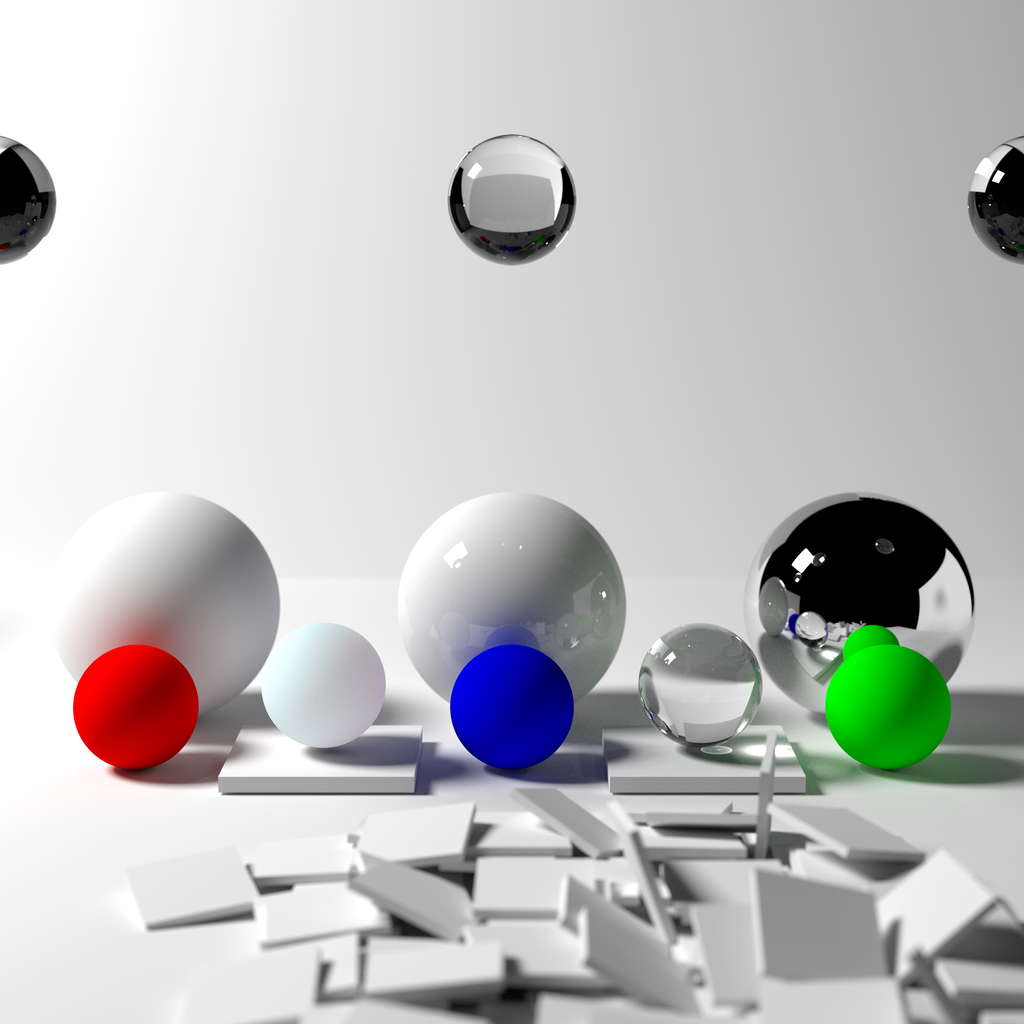
\includegraphics[width=0.7\textwidth]{images/Path_tracing.png}
      \caption*{Path Tracing creates more realistic images}
    \end{figure}
  \end{center}
\end{frame}

\begin{frame}{The Rendering Equation}
  \begin{center}
    \begin{mathbox}{The Holy Grail of Computer Graphics}
      \small
      \begin{align*}
        L_o(\mathbf{P}, \omega_o, \lambda) = L_e(\mathbf{P}, \omega_o, \lambda) + \int_\Omega f(\mathbf{P}, \omega_i, \omega_o, \lambda) L_i(\mathbf{P}, \omega_i, \lambda) (\mathbf{N} \cdot \omega_i) d\omega_i
      \end{align*}
    \end{mathbox}
  \end{center}

  \begin{columns}
    \begin{column}{0.6\textwidth}
      \scriptsize
      \textbf{Components:}
      \begin{itemize}
        \item $L_i$ = Incoming radiance, $L_o$ = Outgoing radiance
        \item $L_e$ = Emitted light
        \item $f$ = BRDF (material property)
        \item $\Omega$ = Hemisphere of directions
        \item $\omega_i$ = Incoming direction, $\omega_o$ = Outgoing direction
        \item $\mathbf{P}$ = Point on surface, $\mathbf{N}$ = Surface normal
        \item $\lambda$ = Wavelength
      \end{itemize}
    \end{column}
    \begin{column}{0.4\textwidth}
      \scriptsize
      \begin{tikzpicture}[scale=0.7]
        \draw[thick, ObjectColor] (-1,0) -- (3,0);
        \fill[AccentColor] (1,0) circle (3pt);
        \node[below] at (1,-0.1) {$\mathbf{P}$};

        \draw[->, SecondaryColor, thick] (1,0) -- (1,1.5);
        \node[right] at (1,1.5) {$\mathbf{N}$};

        \begin{scope}[shift={(1,0)}]
          \draw[dashed] (-1.2, 0) arc [start angle=180, end angle=0, radius=1.2];
          \draw[->, lightray, thick] (0,0) -- (30:1.2);
          \draw[->, lightray, thick] (0,0) -- (75:1.2);
          \draw[->, lightray, thick] (0,0) -- (60:1.2);
          \draw[->, lightray, thick] (0,0) -- (100:1.2);
          \draw[->, lightray, thick] (0,0) -- (120:1.2);
          \node[lightray, right] at (30:1.2) {$\omega_i$};
          \draw[->, RayColor, thick] (0,0) -- (150:1.2) node[left] {$\omega_o$};
        \end{scope}

        \node[above] at (1,1.8) {\small Hemisphere $\Omega$};
      \end{tikzpicture}
    \end{column}
  \end{columns}

  \begin{conceptbox}{The Challenge}
    \footnotesize
    \textbf{Integral:} Infinite directions to sample → Monte Carlo approximation needed
  \end{conceptbox}
\end{frame}

\begin{frame}{Path Tracing vs Ray Tracing}
  \begin{columns}
    \begin{column}{0.5\textwidth}
      \begin{raybox}{Ray Tracing Limitations}
        \begin{itemize}
          \item Perfect mirrors only
          \item Direct illumination focus
          \item Limited global effects
          \item Deterministic sampling
        \end{itemize}
      \end{raybox}
    \end{column}
    \begin{column}{0.5\textwidth}
      \begin{raybox}{Path Tracing Advantages}
        \begin{itemize}
          \item Physically accurate lighting
          \item Global illumination
          \item Soft shadows, caustics
          \item Unbiased rendering
        \end{itemize}
      \end{raybox}
    \end{column}
  \end{columns}
\end{frame}